% arara: lualatex
% arara: lualatex
% arara: lualatex if found('log', 'undefinede references')

%% arara: clean: {extensions: [aux, fdb_latexmk, fls, listing, log, out, pdf, toc]}

% classe do documento ====================================================
\documentclass{book}


% fontes e cia
\usepackage{euler}
\usepackage{fontspec}
  \setmainfont[Ligatures=TeX]{TeX Gyre Pagella}
  \setsansfont[Ligatures=TeX, Scale=0.9]{Oxygen}
  \setmonofont[Scale=MatchLowercase]{Andika}
  \newfontfamily{\terminal}{Inconsolata Nerd Font Mono}
  \newfontfamily{\caligrafica}{Weddingday Personal Use}
  \newfontfamily{\caligra}{Exmouth}
  \newfontfamily{\initial}{Royal Initialen}
  \newfontfamily{\grega}{FreeSerif}
\usepackage{lettrine}

% linguagem 
\usepackage[brazilian]{babel}

% margens 
\usepackage[a5paper]{geometry}

% matemática 
\usepackage{mathtools}
\usepackage{amsthm, amssymb}

% tabelas e figuras
\usepackage{tabularray}
\usepackage[%
  font={small, sf}, 
  labelfont={bf, sf}
]{caption}
\usepackage{graphicx}
  \graphicspath{ {./figs/} }

% seções & cia
\usepackage{sectsty}
  \allsectionsfont{\color{azulUFRB}\sffamily}
\usepackage{fancyhdr}
  \pagestyle{fancy}
    \lhead[\sffamily\small\thepage~\emoji{crossed-swords}\normalsize]{\sffamily \small\leftmark}
    \rhead[{\sffamily \small \rightmark}]{\sffamily\small~\emoji{crossed-swords}~\thepage\normalsize}
    \lfoot{}
    \cfoot{}
    \rfoot{}


% protusão 
\usepackage{microtype}

% cores
\usepackage{xcolor}
  \definecolor{douradoUFRB}{rgb}{0.929411765, 0.603921569, 0.066666667} 
  \definecolor{azulUFRB}{rgb}{0.160784314, 0.08627451, 0.435294118}

% simbologias e adornos
\usepackage{hologo}
\usepackage{postit}
\usepackage{emoji}
\usepackage{fontawesome5}

% códigos LaTeX 
\usepackage{ProfLycee}

% unidades de medidas
\usepackage{siunitx}

% hiperlinks e metadados
\usepackage{hyperref}
  \hypersetup
  {
    colorlinks   = true,
    linkcolor    = azulUFRB,
    citecolor    = azulUFRB,
    filecolor    = douradoUFRB,
    urlcolor     = douradoUFRB,
    pdfnewwindow = true,
    pdfproducer  = {LuaTeX},
    pdfcreator   = {LaTeX2e com neovim e arara}, 
    pdftitle     = {Microcurso sobre LaTeX (texto de apoio)},
    pdfauthor    = {Ícaro Vidal Freire},
    pdfsubject   = {Minicurso para Semanas de Matemática},
    pdfkeywords  = {tex, latex, lualatex, arara, minicurso, ufrb, math}
  }
 %-----> inserindo pacotes fundamentais
% configurações de título
\title
{%
  \sffamily \bfseries 
  Microcurso sobre \textrm{\hologo{LaTeX}} \\
  \Large (texto de apoio)
}
\author
{%
  \sffamily
  Ícaro Vidal Freire
}
\date
{
  \sffamily
  \the\year
}
 %-----> configurações gerais

% início do documento ====================================================
\begin{document}
% 
  \frontmatter % pré-textuais ---------------------------------------
%
  \maketitle
%
  \thispagestyle{empty}

\begin{center}
  {
    \sffamily \bfseries 
    Microcurso sobre \textrm{\LaTeX} (texto de apoio) \\
  }
  \vspace{1em}
  {
    \sffamily \small 
    Copyright \copyright\ 2023, Ícaro Vidal Freire 
  } \\
  \begin{tblr}{rl}
    \small \faEnvelope[regular] & \small \textsf{icarofreire@ufrb.edu.br} \\ 
    \small \faGithub            & \small \href
                                         {%
                                           https://github.com/icaro-freire/microcurso-LaTeX_texto-de-apoio
                                         }{\sffamily github.com/icaro-freire} \\
    \small \faCode              & \small \textsf{v0.1.0}
  \end{tblr}
\end{center}
 %-------------------> copyright
  
\chapter*{O porquê desse texto}
\label{chap:intro}

\lettrine[lines=3]{\color{azulUFRB} \initial T}{alvez essa seja} a quarta (ou 
quinta, realmente não lembro) tentativa de escrever um texto sobre \hologo{LaTeX} 
que seja sucinto, introdutório e que aponte um caminho seguro para quem deseja 
se aprofundar em referências consolidadas sobre o tema.
Não tenho a pretensão de seja um \textsf{manual} ou \textsf{tutorial} sobre 
\hologo{LaTeX}. 
Ele é apenas um \textsf{texto de apoio} a um microcurso (denomino ``micro''; 
pois, geralmente, é menos do que \qty{4}{h} de curso --- um completo absurdo, 
diga-se de passagem \emoji{smile}).
A leitura de um manual/tutorial consolidado é \textsf{fundamental} se você 
deseja usar esse sistema de composição tipográfica em seus textos (farei algumas 
indicações mais adiante). 

\begin{center}
  \begin{PostItNote}[Render=tikz, Color=douradoUFRB]
    \sffamily
    Embora você possa ler esse texto e fruir de uma noção inicial do uso do 
    \textrm{\hologo{LaTeX}}, o ideal seria a participação no microcurso. 
  \end{PostItNote}
\end{center}

Do exposto, vamos delinear alguns procedimentos para que a leitura desse texto 
seja a mais proveitosa possível. 

É meu desejo que, ao final do microcurso (ou desta leitura) você esteja apto a 
reproduzir a seguinte estrutura de um artigo:

\begin{center}
  \linkExt{%
    https://icaro-freire.github.io/projeto_artigo/main.pdf
  }{Artigo Genérico Isento de Sentido}
\end{center}

Obviamente, o conteúdo do artigo (cômico em certas partes) em questão não está 
estruturado de forma linear. 
Essa não foi a intenção. 
O desejo é que você saiba reproduzir a \textsf{estrutura} de um artigo genérico 
em Matemática: referências cruzadas; estruturas de teoremas, proposições, 
definições, etc.; inserção de figuras; estruturas matemáticas básicas como 
matrizes, potências, integrais, derivadas, etc.; alinhamento de equações; 
nomeação de equações; lista; tabelas e referências bibliográficas.

Para tanto, a organizaçao desse texto é a seguinte: darei uma visão geral das 
estrururas e comandos básicos usados no artigo; e, depois, o ``passo a passo''
da construção do artigo citado. 

Mais especificamente:

\begin{description}
  \item[\textbs{Capítulo~\ref{cap:latex}}] 
       Basicamente, desejo abordar as nucances do que seja o \hologo{LaTeX}; 
       sua filosofia; estruturação da classe \textit{article}; e, como podemos 
       organizar os mais diferentes arquivos numa produção de um artigo nesse 
       sistema. 
  \item[\textbs{Capítulo~\ref{cap:modo-texto}}] 
       A intenção neste capítulo é expor alguns dos comandos ou ambientes 
       frequentemente usados no \textsf{modo texto}: tamanho e estilo de fontes;
       uso de tabelas e figuras; configurações das legendas; referências cruzadas; 
       referências no padrão da \textsc{abnt}; como criar novos comandos; etc. 
  \item[\textbs{Capítulo~\ref{cap:modo-math}}] 
       Neste penúltimo capítulo, pretendo abordar estruturas e ambientes para 
       escrita matemática. 
       Obviamente é um tópico bastante amplo e que apenas será tangenciado;
       na esperança de que os leitores percebam a beleza que esse sistema pode 
       oferecer na construção de textos que envolvam espressões matemáticas 
       (embora tal beleza não seja exclusiva ao modo matemático).
  \item[\textbs{Capítulo~\ref{cap:passo-a-passo}}] 
       Por fim, mostro o passo a passo de como construir o \textsf{Artigo Genérico}
       citado mais acima. 
\end{description}

É importante ressaltar que, para esse microcurso, usaremos uma a plataforma 
\textit{online} \linkExt{https://www.overleaf.com/}{Overleaf} para escrevermos o 
\textsf{Artigo Genérico}. 
Tal plataforma disponibiliza muitas ferramentas que, no meu entendimento, pode 
ser icentivadoras num primeiro contato com o \hologo{LaTeX} (não precisamos 
lidar com erros de instalação; a renderização do texto pode ser quase automática; 
diversos \textit{templates} que podem ser acessados com muita dacilidade; etc.). 
Para saber mais sobre essa plataforma, inclusive como configurá-la para nossos 
objetivos, acesse o Apêndice~\ref{apend:overleaf}.

Espero que esse esforço seja útil para aqueles que buscam conhecer esse 
sistema de composição tipográfica tão surpreendente. 

\begin{flushright}
  Amargosa, \today. 

  \caligrafica \LARGE
  Ícaro Vidal Freire
\end{flushright}




 %--------------> introdução
%
  {\sffamily \tableofcontents}
%
  \mainmatter % principais ------------------------------------------
%
  \chapter{O que é o \textrm{\LaTeX}?}
\label{cap:latex}

\lettrine[lines=3]{\color{azulUFRB} \initial R}{esumidamente}, o \hologo{LaTeX} 
é um \textsf{sistema} de preparação de documentos para composição tipográfica 
de alta qualidade. 
Mas\ldots\ o que isso realmente siginifica?  

\section{Arte e Tecnologia juntos} %--------------------------------------

Quando penso numa definição sobre \latex\ geralmente associo a uma função de 
várias variáveis (sou matemático, o que posso fazer? \emoji{grin}). 
E, duas dessas variáveis são fundamentais: \textit{engine} e \textit{format}.
O termo \textit{engine} pode ser traduzido de diversas formas, mas entendo como 
\textsf{mecanismo} ou \textsf{motor}; da mesma forma, o termo \textit{format}, 
pode significar \textsf{formato} ou \textsf{linguagem}. 
Tais conjuntos de ferramentas, são usadas para produzir um arquivo final de alta 
qualidade tipográfica (hoje, geralmente, com extensão \texttt{.pdf}). 
Então, ao usarmos o \latex, escrevemos um \textsf{manuscrito} que mistura texto 
com códigos; e, depois de um processo de \textsf{composição} (que, geralmente 
falamos \textsf{compilação}, por conta de aspectos ligados à computação) é gerado, 
dentre outras coisas, um arquivo final com qualidade já de impressão. 

Falando nisso \ldots\ você ainda lembra o que é um \textsf{manuscrito} e do 
processo que era produzir um texto com qualidade suficiente para imperssão? 
Na época em que se usava papel e caneta, um professor de matemática, por exemplo, 
escrevia suas notas de aulas e as usava até o papel ficar amarelado. 
Eventualmente, um colega descobre essas notas e as usa quando ministra a mesma 
disciplina, posteriormente. 
Então, afirma que essas preciosas notas deveriam ser publicadas. 
Convencido, o professor que as escreveu procura uma editora e apresenta o 
manuscrito (que possivelmente passou por um processador de texto padrão). 
A editora, então, escolhe as fontes para o texto e símbolos matemáticos; o 
espaçamento adequado; qual tamanho de papel; como será a disposição do texto 
nesta folha; passa por outro programa que melhora o texto digitado no 
processador de texto padrão; etc.; para depois enviar para impressão. 
Todo esse processo é o que se chama de \textsf{composição tipográfica}.

\begin{center}
  \begin{PostItNote}[Render=tikz, Color=douradoUFRB]
    \sffamily
    Podemos afirmar, portanto, que o \latex\ é um conjunto (sistema) estruturado 
    de ferramentas que envolve um \textbs{formato} de escrita específico e uso 
    de um \textbs{mecanismo} para \textbs{compor tipograficamente} um manuscrito 
    com qualidade profissional. 
  \end{PostItNote}
\end{center}

Apenas por curiosidade, a Figura~\ref{fig:phd} mostra como era comum, numa época 
anterior ao \latex\ ou a sistemas tipográficos eletrônicos rudimentares, escrever 
(literalmente) \textsf{à mão}, as equações com simbologias específicas. 

\begin{figure}[!htbp]
  \centering
  \caption{Página 33 da tese de doutorado de Richard Feynman}
  \label{fig:phd}
  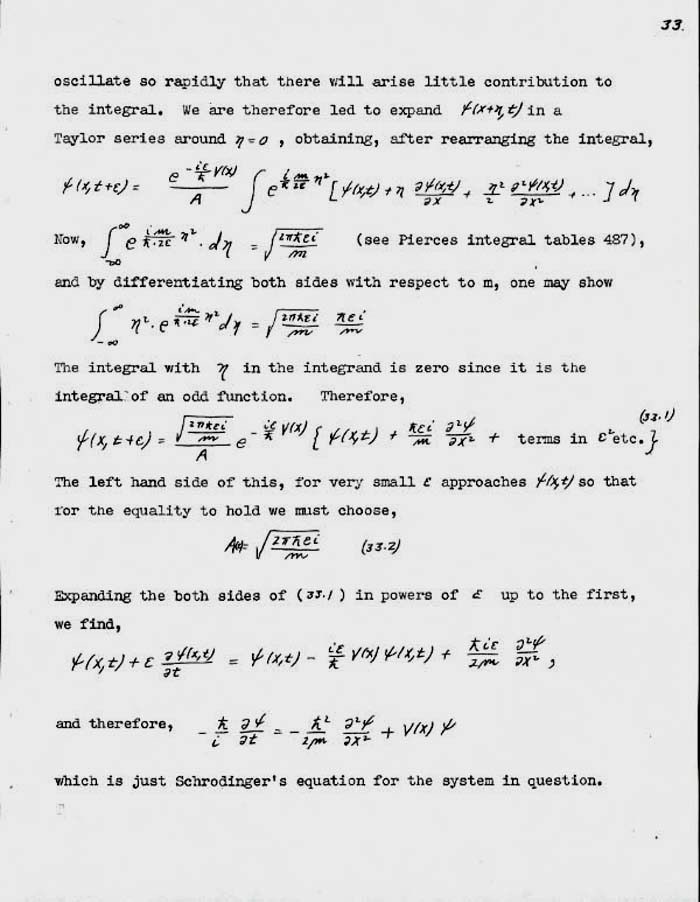
\includegraphics[width = \textwidth]{phd33} \\
  {
  \small \sffamily
  \textsf{Fonte:} \href{https://ysfine.com/feynman/fthesis.html}{https://ysfine.com/feynman/fthesis.html}
}
\end{figure}

O nome \latex\ é uma junção de dois outros: \hologo{La} + \TeX. 
O primeiro, veio de \texttt{\textbf{La}}mport, que é o sobrenome do matemático e 
cientista da computação  estadunidense chamado \textsf{Leslie B. Lamport}, que 
na década de 80 criou um conjunto bem estruturado de \textsf{macros} (a grosso 
modo, pense num conjunto de mapeamentos/atalhos de outros comandos mais básicos, 
denominados \textsf{primitivos}) para uma linguagem de programação exclusivamente 
voltada à composição tipográfica: o \TeX. 
Portanto, o \latex\ é uma linguagem de \textsf{marcação} pra uma linguagem de 
\textsf{programação} denominada \TeX. 
O nome \TeX\ é uma junção de três letras gregas: $\tau$ (\textsf{tau}), 
$\varepsilon$ (\textsf{epsilon}) e $\chi$ (\textsf{chi}) --- esta última, lê-se 
``ki''; e possui a mesma raíz etimológica das palavras \textsf{arte} ({\grega τέχνη}) 
e \textsf{tecnologia} ({\grega τεχνολογία}). 
Ou seja, o autor dessa linguagem de programação, propositalmente, escolheu uma 
palavra que expressasse uma ideia de beleza (tal como a arte da {\caligra \Large Caligrafia})
e tecnologia (pois usou e usa os mais sofisticados algorítimos para composição 
tipográfica).
O leve deslocamento para baixo da letra \texttt{E}, foi para deixar claro que 
trata-se de composição tipográfica. 

A história do \latex\ é indissasociável do \TeX. 
E, a história deste último é bem peculiar: \textsf{Donald Ervin Knuth}, no final 
da década de 1970, recebeu as primeiras amostras de seu próprio livro de 
computação, \textit{The Art of Computer Programming}, produzido por um novo 
sistema tipográfico de sua editora. 
O resultado não agradou ao Knuth que, como cientista da computação, compreendeu 
que a disposição tipográfica de um texto é, em essência, um processo estruturado 
e lógico de preenchimento ou não de tinta no papel. 
E, isso poderia ser traduzido em linguagem computacional: 0 (sem tinta) ou 1 (com tinta). 
Em resumo: criou uma linguagem de programação voltada à composição tipográfica, 
que viria revolucionar a escrita de textos impressos, em especial os textos que 
envolviam Matemática (mas, não exclusivamente ela), porque não encontrou beleza 
no resultado tipográfico de um de seus livros. \emoji{joy}\emoji{upside-down-face}
O próprio Knuth criou um conjunto de macros para o \TeX, denominado \textit{Plain \TeX}, 
para que pudesse usar alguns conjuntos de comandos que frequentemente precisava. 
Mas, Lamport estruturou os conjuntos de macros de maneira tão organizada e eficiente 
que logo se popularizou entre os matemáticos (ou quem precisava escrever algo que 
envolvesse principalmente expressões matemáticas). 
Você pode ler mais sobre a história do \TeX\ neste \textit{link}: 
\linkExt{https://tug.org/whatis.html}{History of TeX}. 

Entretanto, ainda havia limitações em muitos aspectos no \latex: tanto no 
conjunto de macros, quanto nos mecanismos associados à composição tipográfica. 
Outras versões foram surgindo e essas limitações sendo sanadas. 
A última versão modificada pelo próprio Lamport foi a \hologo{LaTeX}~$2.09$. 
Depois disso o projeto passou para um grupo de desenvolvedores que trouxeram 
significativas mudanças estruturais, mas sempre com o princípio de manter a 
compatibilidade naquilo que era possível das versões anteriores. 
Assim, em 1994, surge o \hologo{LaTeX2e} (o $\varepsilon$, provavelmente aparece aí 
para passar a ideia de que a modificação foi mínima/pequena --- fazendo uma 
alusão a ideia do $\varepsilon$ na definição de limites, em Matemática)
\footnote{ 
  $ \lim\limits_{x \to a} f(x) = L$ se para todo $ \varepsilon > 0 $ dado, existir 
  $ \delta > 0 $, tal que a seguinte afirmação é verdadeira:
  \[
    \vert x - a \vert < \delta \Rightarrow \vert f(x) - L \vert < \varepsilon,
  \]
  ou seja, $L$ é o \textsf{limite} de $f(x)$ quando $x$ tende ao real $a$, se a 
  distância de $ f(x) $ ao número real $ L $ é ``tão pequena quanto se queira'', 
  desde que $ x $ esteja ``suficientemente próximo'' de $a$.
} que continua sendo a versão atual (\the\year). 
Havia uma possibilidade de uma nova reestruturação, agora mais significativa, no 
\hologo{LaTeX2e}, passando para uma versão denominada \latex$3$. 
Entretanto, por conta do princípio da compatibilidade para versões anteriores, 
essa ideia foi abandonada e decidiu-se modernizar gradualmente o \hologo{LaTeX2e}. 
Você pode saber mais sobre o \LaTeX 3 e seus desdobramentos atuais no \textit{link}:
\linkExt{https://www.latex-project.org/latex3/}{The \LaTeX\ Project}.

\begin{center}
  \begin{PostItNote}[Render=tikz, Color=douradoUFRB]
    \sffamily
    Note que, atualmente, quando falamos ``\latex'', estamos implicitamente 
    falando da versão \textrm{\hologo{LaTeX2e}}; mas, por simplicidade, usaremos 
    apenas a primeira notação.
  \end{PostItNote}
\end{center}

\section{Mais sobre os mecanismos de composição tipográfica}

A modernização sempre acompanhou o \latex. 
A saída final de um documento, no início do \latex, era em \texttt{DVI} 
(\textit{device independent file format}).  
O \texttt{PDF} foi criado apenas em 1992 e, com sua popularidade, o mecanismo 
de composição do \latex\ foi modificado. 
Inicialmente, havia um conversor do \texttt{DVI} para \texttt{PDF}; depois, em 
1999, surgiu o \hologo{pdfTeX} que produzia o \texttt{PDF} final diretamte, além 
de muitas outras funcionalidades: melhora na quebra de parágrafos; melhora 
significativa no processo de deixar o texto ``justificado''; etc. 


\begin{center}
  \begin{PostItNote}[Render=tikz, Color=douradoUFRB]
    \sffamily
    Como pronunciamos a palavra \latex ?
    Existem duas formas aceitáveis: ou {\tt La-Téc}, ou {\tt Lei-Téc}. 

    Evite falar {\tt La-Técks}, ou pior {\tt Lá-Tecks} (que é aquela seiva 
    branca encontrada em algumas árvores). 
    Além disso, escreva LaTeX, quando não puder escrever \latex 
    --- evite Latex.
  \end{PostItNote}
\end{center}

\begin{figure}[!htbp]
  \centering
    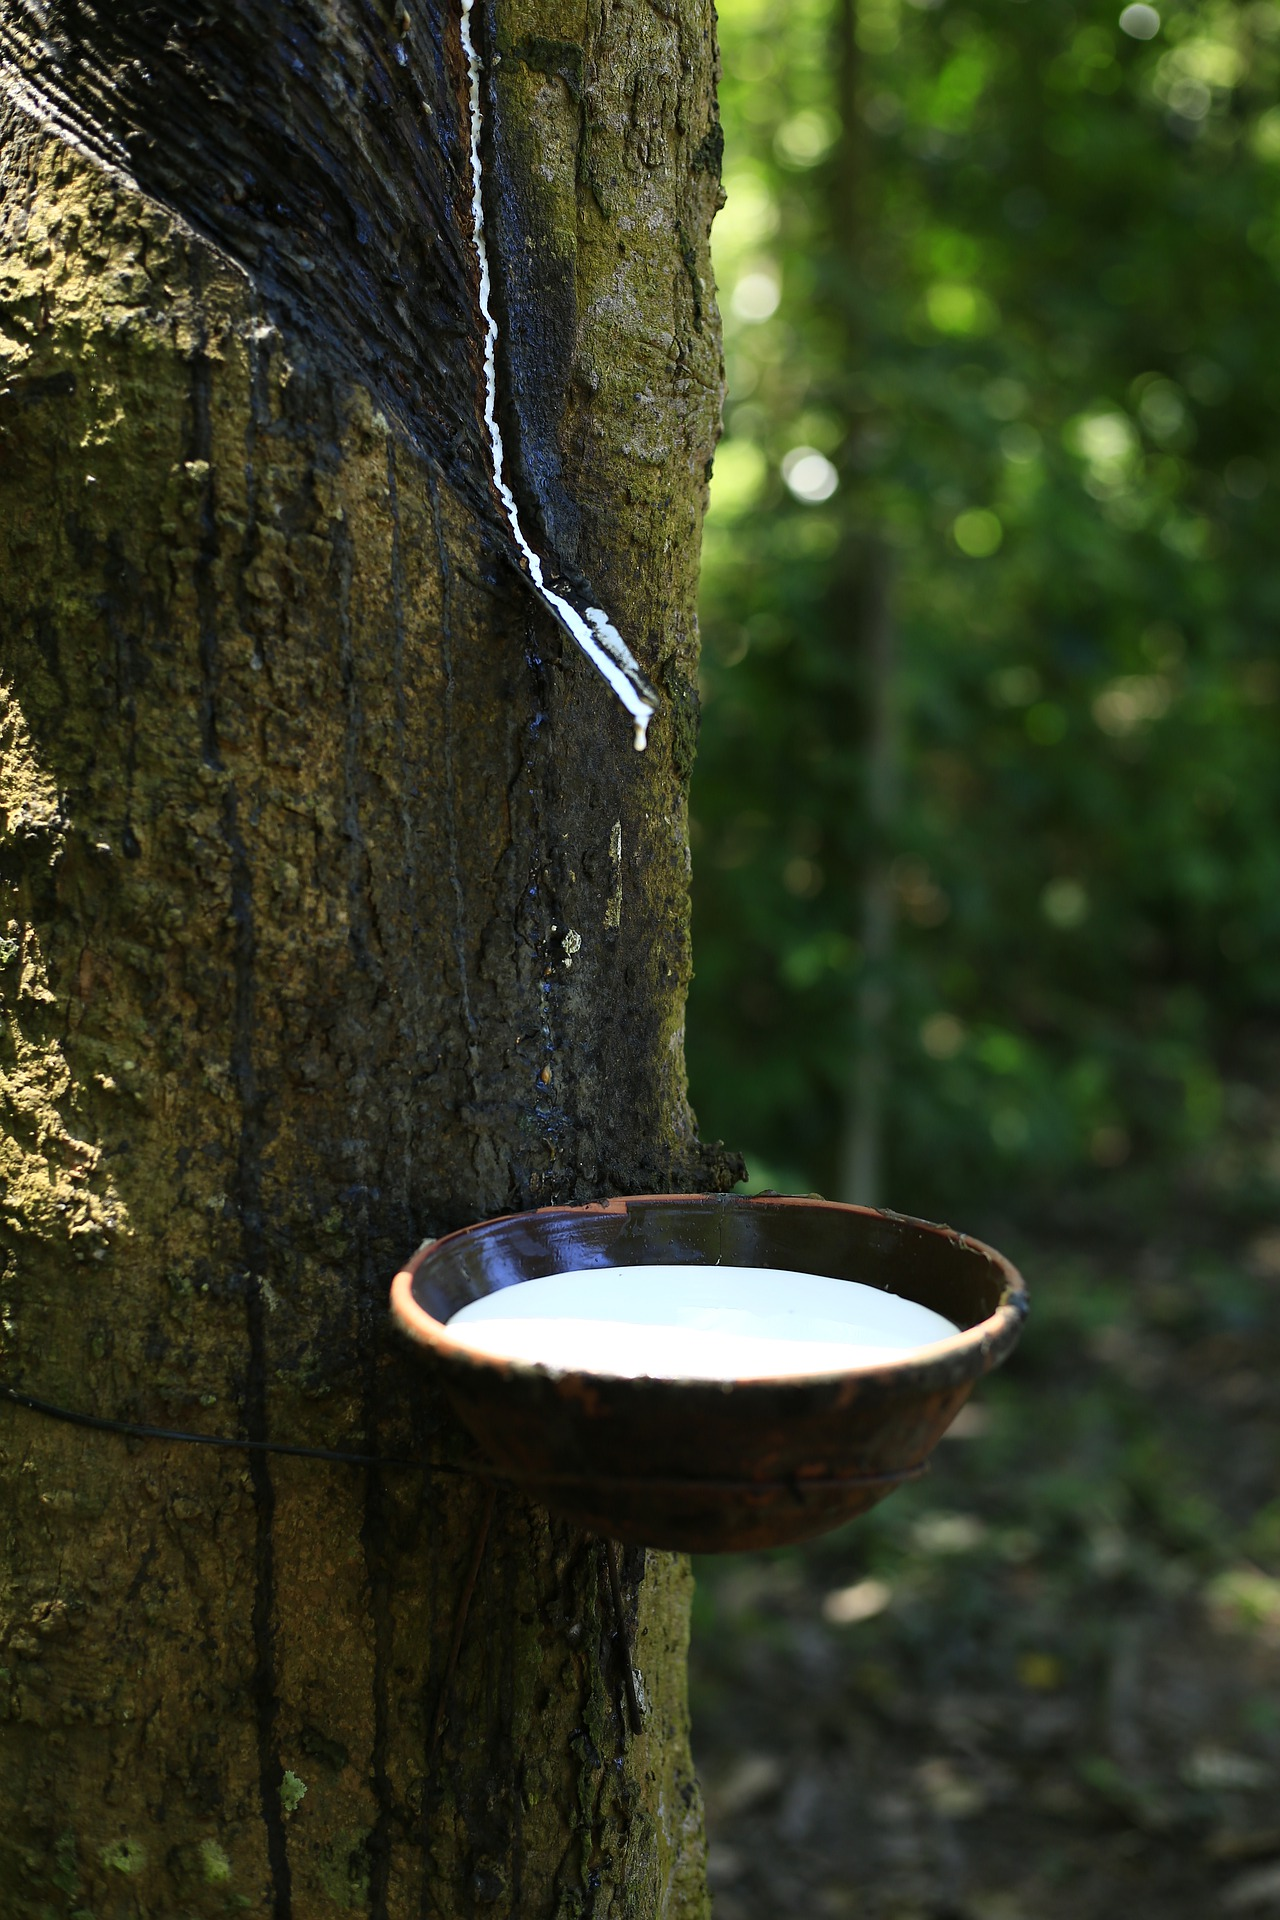
\includegraphics[width=0.4\textwidth]{seringueira}
  \caption{Isso é Látex, não \textrm{\hologo{LaTeX}}}
\end{figure}
 %----------------> capítulo 01
  
\chapter{Algo sobre o Modo Texto}
\label{cap:modo-texto}

Lorem ipsum dolor sit amet, officia excepteur ex fugiat reprehenderit enim labore culpa sint ad nisi Lorem pariatur mollit ex esse exercitation amet. Nisi anim cupidatat excepteur officia. Reprehenderit nostrud nostrud ipsum Lorem est aliquip amet voluptate voluptate dolor minim nulla est proident. Nostrud officia pariatur ut officia. Sit irure elit esse ea nulla sunt ex occaecat reprehenderit commodo officia dolor Lorem duis laboris cupidatat officia voluptate. Culpa proident adipisicing id nulla nisi laboris ex in Lorem sunt duis officia eiusmod. Aliqua reprehenderit commodo ex non excepteur duis sunt velit enim. Voluptate laboris sint cupidatat ullamco ut ea consectetur et est culpa et culpa duis.

 %----------------> capítulo 01
  
\chapter{Algo sobre o Modo Matemático}
\label{cap:modo-math}

Lorem ipsum dolor sit amet, officia excepteur ex fugiat reprehenderit enim labore culpa sint ad nisi Lorem pariatur mollit ex esse exercitation amet. Nisi anim cupidatat excepteur officia. Reprehenderit nostrud nostrud ipsum Lorem est aliquip amet voluptate voluptate dolor minim nulla est proident. Nostrud officia pariatur ut officia. Sit irure elit esse ea nulla sunt ex occaecat reprehenderit commodo officia dolor Lorem duis laboris cupidatat officia voluptate. Culpa proident adipisicing id nulla nisi laboris ex in Lorem sunt duis officia eiusmod. Aliqua reprehenderit commodo ex non excepteur duis sunt velit enim. Voluptate laboris sint cupidatat ullamco ut ea consectetur et est culpa et culpa duis.

 %----------------> capítulo 01
  
\chapter{Passo a passo}
\label{cap:passo-a-passo}

Lorem ipsum dolor sit amet, officia excepteur ex fugiat reprehenderit enim labore culpa sint ad nisi Lorem pariatur mollit ex esse exercitation amet. Nisi anim cupidatat excepteur officia. Reprehenderit nostrud nostrud ipsum Lorem est aliquip amet voluptate voluptate dolor minim nulla est proident. Nostrud officia pariatur ut officia. Sit irure elit esse ea nulla sunt ex occaecat reprehenderit commodo officia dolor Lorem duis laboris cupidatat officia voluptate. Culpa proident adipisicing id nulla nisi laboris ex in Lorem sunt duis officia eiusmod. Aliqua reprehenderit commodo ex non excepteur duis sunt velit enim. Voluptate laboris sint cupidatat ullamco ut ea consectetur et est culpa et culpa duis.

 %----------------> capítulo 01
%
  \appendix % apêndices ---------------------------------------------
  \chapter{Overleaf}
\label{apend:overleaf}

Lorem ipsum dolor sit amet, officia excepteur ex fugiat reprehenderit enim labore culpa sint ad nisi Lorem pariatur mollit ex esse exercitation amet. Nisi anim cupidatat excepteur officia. Reprehenderit nostrud nostrud ipsum Lorem est aliquip amet voluptate voluptate dolor minim nulla est proident. Nostrud officia pariatur ut officia. Sit irure elit esse ea nulla sunt ex occaecat reprehenderit commodo officia dolor Lorem duis laboris cupidatat officia voluptate. Culpa proident adipisicing id nulla nisi laboris ex in Lorem sunt duis officia eiusmod. Aliqua reprehenderit commodo ex non excepteur duis sunt velit enim. Voluptate laboris sint cupidatat ullamco ut ea consectetur et est culpa et culpa duis.

  
\begin{figure}[!h]
  \centering
    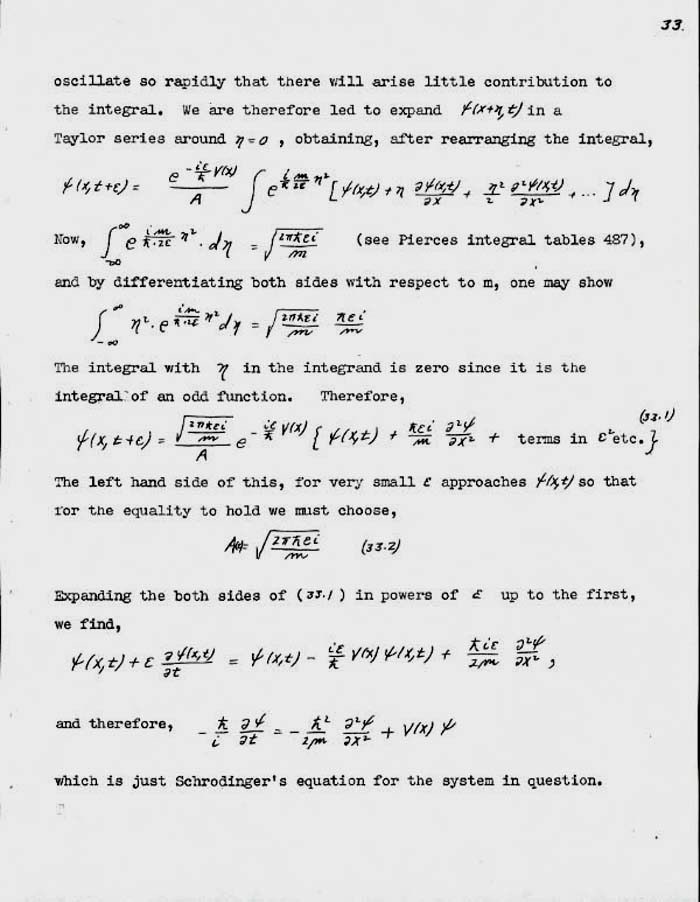
\includegraphics[width = \textwidth]{phd33}
    \caption{Página 33 da tese de doutorado de Richard Feynman}
\end{figure}

%
%
  \backmatter % bibliografia ----------------------------------------
%
\end{document}
%=========================================================================
